%! TEX root = ../main.tex

    \exam{Manipulation d'images, requêtes SQL}{08-04-2023}

    Les barèmes sont indicatifs et pourront être reconsidérés.

    \section*{Requêtes SQL (12 points)}

    On dispose d'une base de données \textsc{Research} d'articles scientifiques. Dans cette base de données on trouve les tables \texttt{publication} et \texttt{author}. \autoref{tab:research} représente ces tables et leurs premiers enregistrements. Les colonnes formant la clef primaire d'une table sont marquées d'une étoile $ \star $.

    \begin{table}[h!]
        \centering
        \subfloat[\texttt{publication} donne des informations sur un article de recherche]{
            \begin{tabular}{|p{5cm}lll|}
                \hline
                \texttt{Title}                                            & \texttt{DOI}$ \star $           & \texttt{Field}     & \texttt{Year} \\ \hline
                "Rayons émis par les composés de l’uranium et du thorium" & "10.1080/028418699432509"       & "Physics"          & 1898          \\
                "Protein measurement with the folin phenol reagent."      & "10.1016/S0021-9258(19)52451-6" & "Biology"          & 1951          \\
                "Computing Machinery and Intelligence."                   & "10.1093/mind/LIX.236.433"      & "Computer Science" & 1950          \\
                "Über Gravitationswellen"                                 & "10.1007/978-3-662-57411-9\_17" & "Physics"          & 1918          \\ \hline
            \end{tabular}
        } \hfill %
        \subfloat[\texttt{author} donne des informations sur les auteur.ice.s d'un article]{
            \begin{tabular}{|lllp{5cm}|}
                \hline
                \texttt{Name}$ \star $ & \texttt{FirstName}$ \star $ & \texttt{Article}$ \star $                    & \texttt{Rank}                                   \\
                                       &                             & Clef étrangère pour \texttt{publication.DOI} & Rang dans la contribution de l'auteur.ice à l'article \\
                \hline
                Curie                  & Marie                       & "10.1080/028418699432509"                    & 1                                                     \\
                Lowry                  & Oliver                      & "10.1016/S0021-9258(19)52451-6"              & 1                                                     \\
                Rosebrough             & Nira                        & "10.1016/S0021-9258(19)52451-6"              & 2                                                     \\
                Farr                   & Lewis                       & "10.1016/S0021-9258(19)52451-6"              & 3                                                     \\
                Randall                & Rose                        & "10.1016/S0021-9258(19)52451-6"              & 4                                                     \\
                Turing                 & Alan                        & "10.1093/mind/LIX.236.433"                   & 1                                                     \\
                Einstein               & Albert                      & "10.1007/978-3-662-57411-9\_17"              & 1                                                     \\
                \hline
            \end{tabular}
        }
        \caption{Tables de la base de données \textsc{Research}}
        \label{tab:research}
    \end{table}

    \ques Rédiger une requête SQL pour obtenir les informations suivantes
    \ssques (2 point) Les titres de tous les articles.
    \ssques (2 point) Les titres et années de publication des 5 plus vieux articles.
    \ssques (2 point) Le nombre d'articles publiés après 1980.
    \ssques (2 point) Le titre des articles publiés par Marie Curie.
    \ssques (2 point) Le nom des chercheuses et chercheurs qui ont été auteur.ice principal.e d'un papier de biologie au XXIème siècle, et le titre du ou des papiers correspondant.
    \ssques (2 point) Le nom des chercheuses et chercheurs qui ont collaboré avec Alan Turing.

    \section*{Manipulation d'image (18 points)}

    Dans cette exercice, on suppose que les images vous sont fournies sous forme d'un tableau \texttt{numpy}. De même, lorsqu'on demande de créer une image, on attend juste sa représentation comme tableau \texttt{numpy}. On ne s'intéresse qu'à des images en noir et blanc.

    Soit $ M $ une image de dimension $ m \times n $ (vue comme une matrice de $ M_{m,n}(\Z) $).

    \ques On note $ M^{\leftrightarrow} $ la réflexion horizontale de $ M $. Par exemple, la réflexion horizontale de l'image \autoref{fig:normal} est \autoref{fig:hflip}.
    \ssques (1 point) Quelle est la dimension de $ M^{\leftrightarrow} $ ?
    \ssques (1 point) Exprimer $ M^{\leftrightarrow}_{i,j} $ en fonction des coefficients de $ M $.
    \ssques (3 point) Écrire une fonction \mintinline{python}{reflexion_horizontale(img)} qui prend en argument une image \texttt{img} et renvoie sa réflexion horizontale.

    \ques On note $ M^T $ la transposée de $ M $. Par exemple, la transposée de l'image \autoref{fig:normal} est l'image \autoref{fig:transpose}.
    \ssques (1 point) Quelle est la dimension de $ M^T $ ?
    \ssques (1 point) Exprimer $ M^T_{i,j} $ en fonction des coefficients de $ M $.
    \ssques (3 point) Écrire une fonction \mintinline{python}{transpose(img)} qui prend en argument une image \texttt{img} et renvoie son image transposée.

    \ques On note $ M^{\updownarrow} $ la réflexion verticale de $ M $. Par exemple, la réflexion verticale de l'image \autoref{fig:normal} est \autoref{fig:vflip}.
    \ssques (1 point) Quelle est la dimension de $ M^{\updownarrow} $
    \ssques (1 point) Exprimer $ M^{\updownarrow}_{i,j} $ en fonction des coefficients de $ M $.
    \ssques (2 point) Montrer que $ (M^{T})^{\leftrightarrow} = (M^{\updownarrow})^T $.
    \ssques (1 point) En déduire que $ ((M^T)^{\leftrightarrow})^T = M^{\updownarrow} $

    \ques (3 points) Déduire des questions précédentes une fonction \mintinline{python}{reflexion_verticale(img)} qui prend en argument une image \texttt{img} et renvoie sa réflexion verticale.

    \begin{figure}[h!]
        \begin{center}
            \null\hfill
            \subfloat[$ M $]{
                \label{fig:normal}
                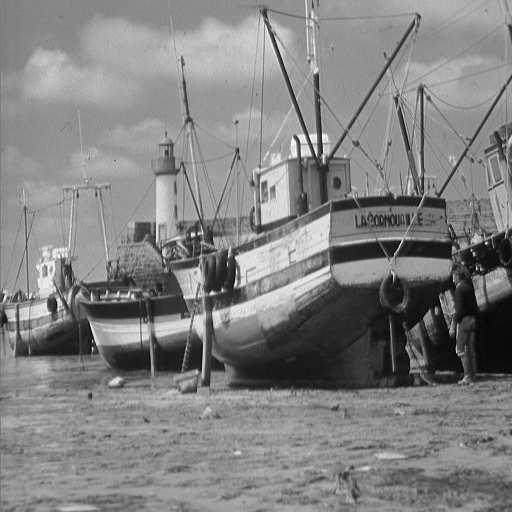
\includegraphics[width=0.35\textwidth]{figures/exams/boat.png}
            } \hfill %
            \subfloat[$ M^{\leftrightarrow} $]{
                \label{fig:hflip}
                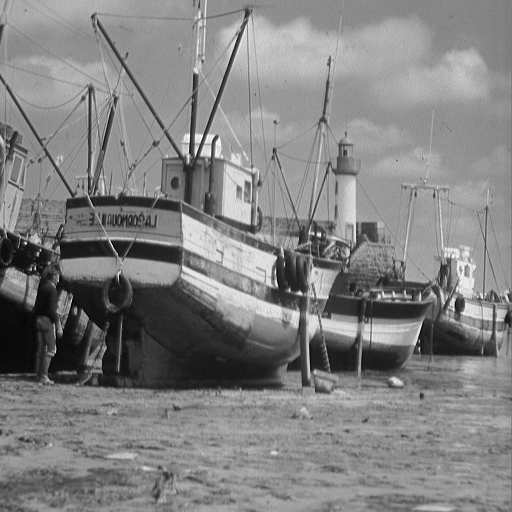
\includegraphics[width=0.35\textwidth]{figures/exams/boat_hflip.png}
            }\hfill\null \\
            \null\hfill
            \subfloat[$ M^{\updownarrow} $]{
                \label{fig:vflip}
                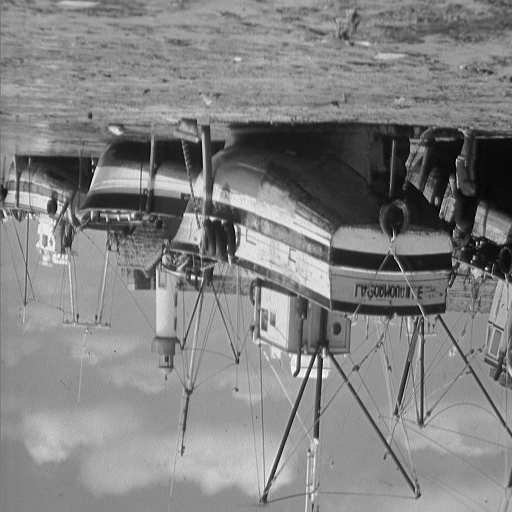
\includegraphics[width=0.35\textwidth]{figures/exams/boat_vflip.png}
            } \hfill %
            \subfloat[$ M^T $]{
                \label{fig:transpose}
                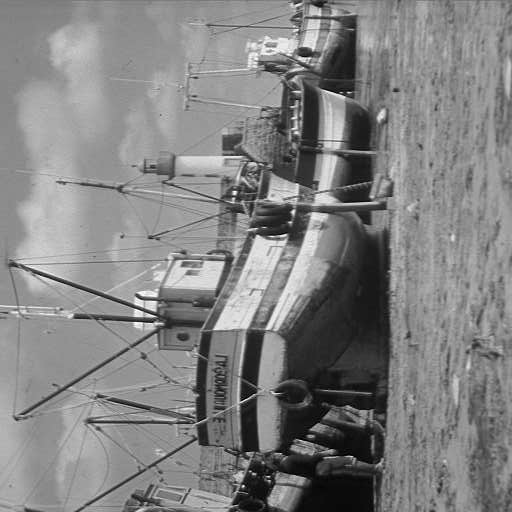
\includegraphics[width=0.35\textwidth]{figures/exams/boat_transpose.png}
            } \hfill\null
        \end{center}
        \caption{Exemple d'opérations géométriques sur une image}
        \label{fig:boat}
    \end{figure}
